\begin{figure}[H]
	\begin{center}
		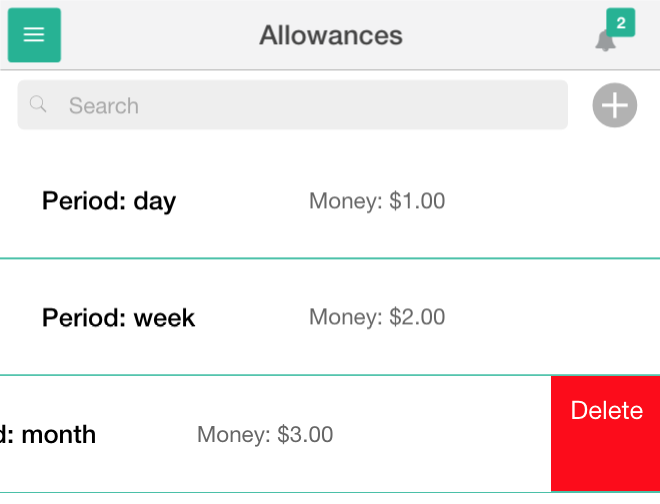
\includegraphics[width=0.5
		\textwidth]{allowances/allowances.png}
	\end{center}
	\caption{Mesadas do utilizador}
	\label{fig:3}
\end{figure}

\begin{figure}[H]
	\begin{center}
		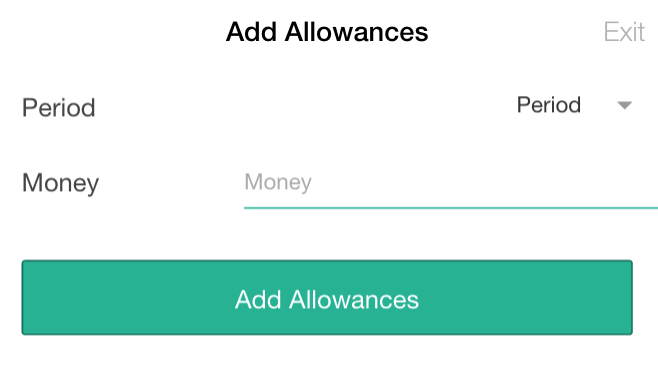
\includegraphics[width=0.5
		\textwidth]{allowances/addAllowances.png}
	\end{center}
	\caption{Adicionar Mesada}
	\label{fig:3_1}
\end{figure}

O ecrã que lista as mesadas (Figura \ref{fig:3}) apresenta as mesadas ativas. Para eliminar uma mesada é necessário arrastar a linha correspondente à mesada e selecionar o botão de apagar. Apenas os pais conseguem adicionar mesadas aos filhos. Para adicionar uma mesada seleciona-se o botão de adicionar no canto superior direito (Figura \ref{fig:3}). Será apresentado um novo ecrã onde é solicitado o período e o montante da mesada, por exemplo, vinte dólares por semana.